\documentclass[Bachelorarbeit.tex]{subfiles}
\begin{document}

\graphicspath{{./figures/hypothesis/}}	%specifying the folder for the figures

\chapter{Hypothesis}
\label{ch:hypothesis}

In this chapter the question of the importance of fully-connectedness for reaching the equilibrium is raised where the question is whether it is really necessary to have a fully-connected network to reach equilibrium or not. We challenge this and claim that a much lower connectivity with a special property is sufficient. First the motivation is presented and the claims behind it are proven mathematically. Then the property is introduced and it is proven that it is necessary to reach theoretical equilibrium. Whether it is sufficient is tested by computer-driven simulation where the results are given in chapter \ref{ch:results}.

\medskip

The initial hypothesis presented in this chapter was conjectured first by the supervisor of this thesis Mr. Hans-Joachim Vollbrecht.

\section{Motivation}
The motivation behind the hypothesis is the fact that according to the double-auction definition - see chapter \ref{ch:theory} - for a match to happen the buyer-price must be larger or equal to the seller-price. This can only be the case if the buyer has a higher optimism-factor than the seller because only then the limit-price of the buyer will be larger than the one of the seller. For a match to occur the limit-price of the buyer has to be strictly larger than the one of the seller as shown below.

\medskip

In figure \ref{fig:MATCHING_BUYER_SELLER_RANGES} the price-ranges of both a seller and buyer are given where l(s) and l(b) denote the limit-price of the seller and buyer respectively which are determined by their optimism-factor \textit{h}. The seller places its offerings in the price-range of [l(s)..pU] as it wants to sell the good above the expected price to make a profit. The buyer places its offerings in the price-range of [pD..l(b)] as it wants to buy the goods below the expected price to make a profit. The resulting matching-range on which the prices can meet - again buyer-price $\geq$ seller-price - is marked by the red rectangle. It is easy to see that a match with these mechanics can occur only if the optimism-factor of the buyer l(b) is strictly higher than the one of the seller l(s).

TODO: replace h(s) and h(b) by l(s) and l(b).

\begin{figure}[H]
	\centering
  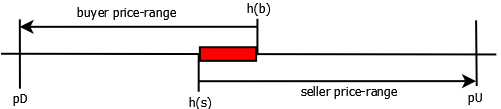
\includegraphics[width=1.0\textwidth, angle=0]{MATCHING_BUYER_SELLER_RANGES.png}
  	\caption{Matching of buyers and sellers price-ranges. The red rectangle marks the matching-range.}
	\label{fig:MATCHING_BUYER_SELLER_RANGES}
\end{figure}

\section{Proof buyer more optimistic than seller}
Proofing that the optimism of a buyer must be greater or equal than the optimism of the seller $h_B \geq h_S$ by using that the limit-price of the buyer must be greater or equal the limit-price of the seller $limit_B \geq limit_S$ and then showing that this can only be the case if $h_B \geq h_S$.

\subsection{Asset/Cash}
$limit_B = h_B \, pU + (1-h_B) \, pD = h_B + \frac{1}{5} - \frac{h_B}{5}$ \\
$limit_S = h_S \, pU + (1-h_S) \, pD = h_S + \frac{1}{5} - \frac{h_S}{5}$

\begin{proof}
\begin{align*}
	limit_S - limit_B \leq 0
	\\ (h_S + \frac{1}{5} - \frac{h_S}{5}) - ( h_B + \frac{1}{5} - \frac{h_B}{5} ) \leq 0
	\\ h_S + \frac{1}{5} - \frac{h_S}{5} - h_B - \frac{1}{5} + \frac{h_B}{5} \leq 0
	\\ 5h_S + 1 - h_S - 5h_B - 1 + h_B \leq 0
	\\ 4h_S - 4h_B \leq 0
	\\ h_S - h_B \leq 0		\tag*{can only hold if $h_B \geq h_S$}
\end{align*}
\end{proof}

\subsection{Bond/Cash}
$limit_B = h_B \, V + (1-h_B) \, pD = h_B \, V + \frac{1}{5} - \frac{h_B}{5}$ \\
$limit_S = h_S \, V + (1-h_S) \, pD = h_S \, V + \frac{1}{5} - \frac{h_S}{5}$

\begin{proof}
\begin{align*}
	limit_S - limit_B \leq 0
	\\ (h_S \, V  + \frac{1}{5} - \frac{h_S}{5}) - ( h_B \, V  + \frac{1}{5} - \frac{h_B}{5} ) \leq 0
	\\ h_S \, V  + \frac{1}{5} - \frac{h_S}{5} -  h_B \, V  - \frac{1}{5} + \frac{h_B}{5} \leq 0
	\\ 5 h_S \, V  + 1 - h_S - 5h_B \, V  - 1 + h_B \leq 0
	\\ 5 h_S \, V - 5h_B \, V - h_S + h_B \leq 0
	\\ 5V(h_S - h_B) - (h_S - h_B) \leq 0	
	\\ (h_S - h_B)(5V - 1) \leq 0			\tag*{$|: (5V-1) \Rightarrow \geq 0 \; | \; V \; [0..1]$}
	\\ h_S - h_B \leq 0
\end{align*}
\end{proof}

\subsection{Asset/Bond}
$limit_B = \frac{h_B + \frac{1}{5} - \frac{h_B}{5}}{h_B \, V + \frac{1}{5} - \frac{h_B}{5}}$ \\
$limit_S = \frac{h_S + \frac{1}{5} - \frac{h_S}{5}}{h_S \, V + \frac{1}{5} - \frac{h_S}{5}}$ \\

\begin{proof}
\begin{align*}
	limit_S - limit_B \leq 0
	\\ \frac{h_S + \frac{1}{5} - \frac{h_S}{5}}{h_S \, V + \frac{1}{5} - \frac{h_S}{5}} - \frac{h_B + \frac{1}{5} - \frac{h_B}{5}}{h_B \, V + \frac{1}{5} - \frac{h_B}{5}} \leq 0
	\\ (h_S + \frac{1}{5} - \frac{h_S}{5})(h_B \, V + \frac{1}{5} - \frac{h_B}{5}) - (h_B + \frac{1}{5} - \frac{h_B}{5})(h_S \, V + \frac{1}{5} - \frac{h_S}{5}) \leq 0													
	\\ substituting \; S = \frac{1}{5} - \frac{h_S}{5}, B = \frac{1}{5} - \frac{h_B}{5}
	\\ (h_S + S)(h_B \, V + B) - (h_B + B)(h_S \, V + S) \leq 0
	\\ h_S \, h_B \, V + h_S \, B + S \, h_B \, V + BS - (h_B \, h_S \, V + h_B \, S + B \, h_S \, V + BS) \leq 0
	\\ h_S \, h_B \, V + h_S \, B + S \, h_B \, V + BS - h_B \, h_S \, V - h_B \, S - B \, h_S \, V - BS \leq 0
	\\ h_S \, B + S \, h_B \, V - h_B \, S - B \, h_S \, V \leq 0
	\\ h_S \, B - h_B \, S + V(h_B \, S - h_S \, B ) \leq 0 
	\\ h_S(\frac{1}{5} - \frac{h_B}{5}) - h_B(\frac{1}{5} - \frac{h_S}{5}) + V(h_B(\frac{1}{5} - \frac{h_S}{5}) - h_S(\frac{1}{5} - \frac{h_B}{5})) \leq 0
	\\ \frac{h_S}{5} - \frac{h_S \, h_B}{5} - \frac{h_B}{5} + \frac{h_B \, h_S}{5} + \frac{h_B \, V}{5} - \frac{h_B \, h_S \, V}{5} - \frac{h_S \, V}{5} + \frac{h_S \, h_B \, V}{5} \leq 0 
	\\ \frac{h_S}{5} - \frac{h_B}{5} + \frac{h_B \, V}{5} - \frac{h_S \, V}{5} \leq 0
	\\ h_S - h_B + h_B \, V - h_S \, V \leq 0 
	\\ h_S( 1 - V ) + h_B( -1 + V ) \leq 0 
	\\ |: (1-V) \Rightarrow \geq 0 \; | \; V \; [0..1]
	\\ h_S + h_B \frac{-(1-V)}{(1-V)} \leq 0
	\\ h_S - h_B \leq 0
\end{align*}
\end{proof}

\section{Proof of monotony of limit-functions}
The property that the optimism-factor of the buyer has to be larger or equal to the one of the seller is not enough for a match to occur. Additionally the limit-function must be monotony increasing in the defined range [0..1] of the optimism-factor \textit{h} because if it is not then no matching would be possible. It is proofed by showing that $limit' > 0$ in the range of \textit{h} = [0..1].

\subsection{Asset/Cash market}
\begin{proof}
\begin{align*}
	limit_{asset} = h \, pU + (1-h) pD		\tag*{pU = 1, pD = 0.2}
	\\ = h + (1 - h)0.2
	\\ = h + \frac{1}{5} - \frac{h}{5}		\tag*{$\frac{\mathrm d}{\mathrm d h}$}
	\\ = 1 - \frac{1}{5}
		&= \frac{4}{5}
\end{align*}
Constant $\Rightarrow$ limit-function is monotony increasing over the real numbers. QED
\end{proof}

\subsection{Bond/Cash market}
\begin{proof}
\begin{align*}
	limit_{bond} = h \, V + (1-h) pD			
	\\ = h \, V + (1 - h)pD
	\\ = h \, V + pD - h\,pD		\tag*{$\frac{\mathrm d}{\mathrm d h}$}
	\\ = V - pD
\end{align*}
V is a constant in range of [0..1] $\Rightarrow$ limit-function is monotony increasing were $V > pD$. QED
\end{proof}

Note that this implies that a bond with face-value \textit{V = pD} cannot be traded as the limit-function is constant for all \textit{h}. This needs to be covered in the implementation.

\subsection{Asset/Bond market}
\begin{proof}
\begin{align*}
	limit_{asset/bond} = \frac{h \, pU + (1-h) pD}{h \, V + (1-h) pD} 				\tag*{pU = 1, pD = 0.2}
	\\ = \frac{h + \frac{1}{5} - \frac{h}{5}}{h \, V + \frac{1}{5} - \frac{h}{5}}	\tag*{$\frac{\mathrm d}{\mathrm d h}$}
	\\ = - \frac{5(V-1)}{(h(5V-1)+1)^2}									\tag*{assume h and V in range [0..1]}
	\\ \Rightarrow 5(V-1) \leq 0
	\\ \Rightarrow (h(5V-1)+1)^2 \geq 0
	\\ \Rightarrow - \frac{5(V-1)}{(h(5V-1)+1)^2} \geq 0 			\tag*{for h and V in range [0..1]}
\end{align*}
first derivation $> 0$ $\Rightarrow$ limit-function is monotony increasing if $h > 0$ and $V > 0$. QED
\end{proof}

Note that the limit-function is undefined in the case of h=0 which should be prevented in the implementation - see chapter \ref{ch:implementation}.

\section{Hypothesis}
\begin{equation}
\begin{split}
\textit{fully-connectedness equilibrium} \iff \\
\forall \: \textit{agent-pairs} \: (a_{1},a_{n}) \: \exists \:  \textit{path} \: P \: \{a_{1}, a_{2}, ... , a_{n-1}, a_{n}\} \: | \: h(a_{i}) < h(a_{i+1})
\end{split}
\end{equation}

\newtheorem{conj}{Conjecture}
\begin{conj}
If and only if for all agents exists a path between two agents in which each visited agent has a larger optimism factor than the previous one then the same equilibrium as in fully-connectedness will be reached.
\end{conj}

\section{Proof of necessity}
In this section it is proven that the given property is \textit{necessary} to reach theoretical equilibrium but it is open to question whether it is \textit{sufficient} or not. This will be investigated by computer-simulation.

\medskip

The most minimal configuration of agents which satisfies the property is a graph of agents where each agent is connected to the agent with the next higher optimism-factor. This is the same as the Ascending-Connected topology - see appendix \ref{app:topologies} - which is the major network of interest in this thesis (besides the fully-connected one) as it is the most minimal topology which satisfies the property.

TODO: hypothese beweisen
1. zeigen dass hypothese auf minimale vernetzung reduziert werden kann bzw. dass diese minimale vernetzung ausreicht. (über den vorhergehenden formal proof und dass limit-prices monoton steigen)
2. zeigen, dass lücken bei minimalster vernetzung an beliebiger stelkle zu widerspruch führt: gleichgewicht wird nicht erreicht. 

\section{Predictions}
The following topologies found in appendix \ref{app:topologies} satisfy the definition of the hypothesis:

\begin{itemize}
\item Fully-Connected
\item Half-Fully connected
\item Ascending-Connected
\item Ascending-Connected with all kind of short-cuts
\item Erdos-Renyi and Watts-Strogatz with the correct parametrization by pure chance.
\end{itemize}

If the hypothesis is valid and the property is sufficient these topologies will reach the equilibrium found in fully-connectedness. All other topologies do not satisfy the necessary property and are expected to clearly fail reaching the equilibrium of the Fully-Connected topology.

\medskip

See chapter \ref{ch:results} and \ref{ch:interpretation} whether the property is sufficient or not. 

\end{document}